\documentclass[tikz,border=6pt]{standalone}
\usepackage[T1]{fontenc}
\usepackage{lmodern}
\usepackage{amsmath}
\usepackage{amssymb}
\usepackage{bm}
\usepackage{xcolor}
\usepackage{tikz}
\usetikzlibrary{arrows.meta,positioning,fit,calc,backgrounds,shapes.multipart,shapes.geometric}

\colorlet{mandalaBlue}{blue!55!black}
\colorlet{mandalaTeal}{teal!55!black}
\colorlet{mandalaGreen}{green!45!black}
\colorlet{mandalaGold}{orange!70!black}
\colorlet{mandalaRed}{red!55!black}
\colorlet{mandalaViolet}{violet!55!black}
\colorlet{mandalaGray}{black!55}
\colorlet{mandalaLight}{black!3}

\tikzset{
  >=Latex,
  font=\sffamily,
  % Color semantics used consistently across all diagrams:
  % mandalaBlue   -> external inputs / sources / configuration
  % mandalaTeal   -> internal data containers / encoded features
  % mandalaGreen  -> geometric or physics-aware transformations
  % mandalaGold   -> model computation or linear-algebra solve stages
  % mandalaViolet -> predicted operator-valued objects and heads
  % mandalaRed    -> optimization / objectives / losses
  titlebox/.style={
    rounded corners=2.5pt,
    fill=mandalaBlue!8,
    draw=mandalaBlue,
    line width=0.8pt,
    inner sep=6pt,
    minimum height=10mm,
    align=center,
    font=\sffamily\bfseries\large
  },
  panel/.style={
    rounded corners=3pt,
    fill=white,
    draw=black!45,
    line width=0.8pt,
    inner sep=5pt
  },
  stage/.style={
    rounded corners=3pt,
    fill=#1!10,
    draw=#1!85!black,
    line width=0.9pt,
    minimum width=32mm,
    minimum height=11mm,
    align=center,
    font=\sffamily\small
  },
  stage/.default=mandalaBlue,
  smallstage/.style={
    rounded corners=2.5pt,
    fill=#1!9,
    draw=#1!80!black,
    line width=0.75pt,
    minimum width=27mm,
    minimum height=8.5mm,
    align=center,
    font=\sffamily\scriptsize
  },
  smallstage/.default=mandalaBlue,
  sidepanel/.style={
    rounded corners=3pt,
    fill=#1!8,
    draw=#1!75!black,
    line width=0.8pt,
    inner sep=5pt,
    align=left,
    font=\sffamily\scriptsize,
    text width=43mm
  },
  sidepanel/.default=mandalaTeal,
  annot/.style={
    font=\sffamily\scriptsize,
    text=mandalaGray,
    align=left
  },
  arrow/.style={
    -{Latex[length=2.6mm,width=1.8mm]},
    line width=0.95pt,
    draw=black!70
  },
  dashedarrow/.style={
    -{Latex[length=2.4mm,width=1.7mm]},
    line width=0.85pt,
    draw=black!65,
    dashed
  },
  softfit/.style={
    rounded corners=4pt,
    draw=black!35,
    fill=black!1,
    line width=0.7pt,
    inner sep=6pt
  },
  lab/.style={
    font=\sffamily\scriptsize\bfseries,
    text=black!75
  },
  tinycode/.style={
    font=\ttfamily\tiny,
    text=black!70,
    align=center
  }
}

\begin{document}
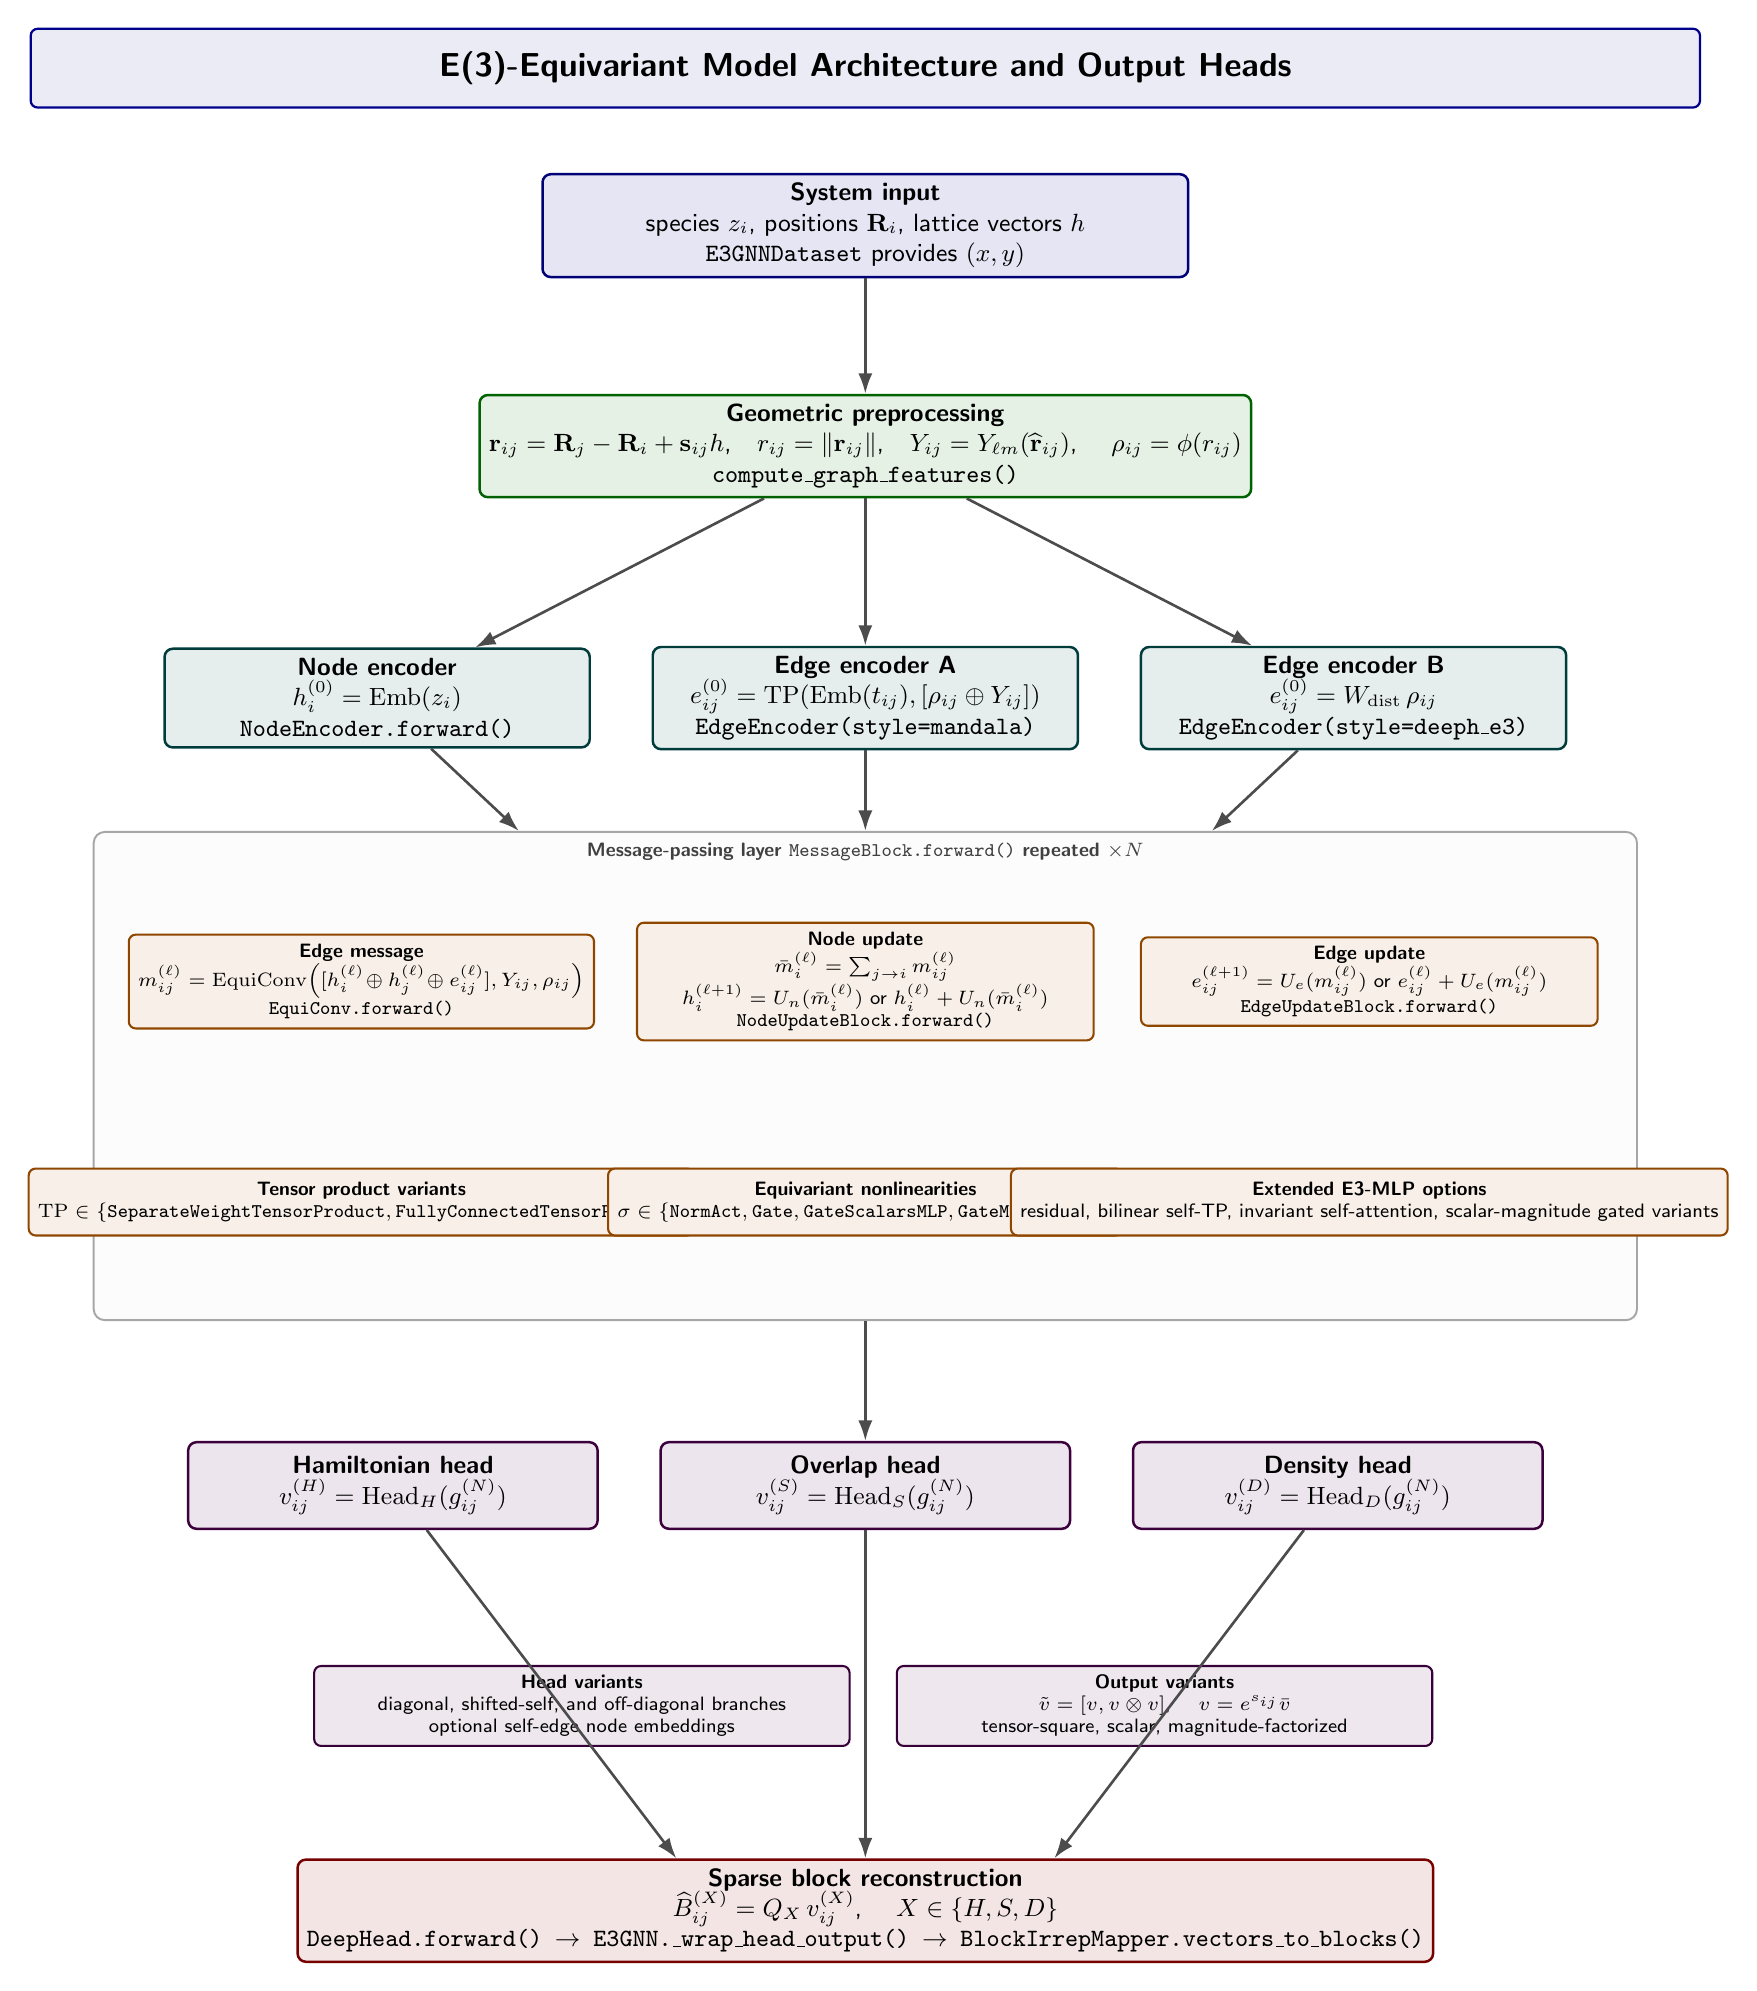
\begin{tikzpicture}[x=1cm,y=1cm]

\node[titlebox, minimum width=21.2cm] (title) at (0,0) {E(3)-Equivariant Model Architecture and Output Heads};

\node[stage=mandalaBlue, minimum width=8.2cm] (input) at (0.0,-2.0)
{\textbf{System input}\\
species $z_i$, positions $\mathbf R_i$, lattice vectors $h$\\
\texttt{E3GNNDataset} provides $(x,y)$};

\node[stage=mandalaGreen, minimum width=9.0cm] (geom) at (0.0,-4.8)
{\textbf{Geometric preprocessing}\\
$\mathbf r_{ij} = \mathbf R_j - \mathbf R_i + \mathbf s_{ij} h$,\quad
$r_{ij}=\|\mathbf r_{ij}\|$,\quad
$Y_{ij}=Y_{\ell m}(\widehat{\mathbf r}_{ij})$, \quad
$\rho_{ij}=\phi(r_{ij})$\\
\texttt{compute\_graph\_features()}};

\node[stage=mandalaTeal, minimum width=5.4cm] (nodeenc) at (-6.2,-8.0)
{\textbf{Node encoder}\\
$h_i^{(0)}=\mathrm{Emb}(z_i)$\\
\texttt{NodeEncoder.forward()}};
\node[stage=mandalaTeal, minimum width=5.4cm] (edgeencA) at (0.0,-8.0)
{\textbf{Edge encoder A}\\
$e_{ij}^{(0)}=\mathrm{TP}\!\left(\mathrm{Emb}(t_{ij}),[\rho_{ij}\oplus Y_{ij}]\right)$\\
\texttt{EdgeEncoder(style=mandala)}};
\node[stage=mandalaTeal, minimum width=5.4cm] (edgeencB) at (6.2,-8.0)
{\textbf{Edge encoder B}\\
$e_{ij}^{(0)} = W_{\mathrm{dist}}\,\rho_{ij}$\\
\texttt{EdgeEncoder(style=deeph\_e3)}};

\draw[arrow] (input) -- (geom);
\draw[arrow] (geom) -- (nodeenc);
\draw[arrow] (geom) -- (edgeencA);
\draw[arrow] (geom) -- (edgeencB);

\node[softfit, minimum width=19.6cm, minimum height=6.2cm] (mpbox) at (0.0,-12.8) {};
\node[lab] at (0.0,-9.95) {Message-passing layer \texttt{MessageBlock.forward()} repeated $\times N$};

\node[smallstage=mandalaGold, minimum width=5.8cm] (mp1) at (-6.4,-11.6)
{\textbf{Edge message}\\
$m_{ij}^{(\ell)}=\mathrm{EquiConv}\!\left([h_i^{(\ell)}\!\oplus h_j^{(\ell)}\!\oplus e_{ij}^{(\ell)}],Y_{ij},\rho_{ij}\right)$\\
\texttt{EquiConv.forward()}};
\node[smallstage=mandalaGold, minimum width=5.8cm] (mp2) at (0.0,-11.6)
{\textbf{Node update}\\
$\bar m_i^{(\ell)}=\sum_{j\to i} m_{ij}^{(\ell)}$\\
$h_i^{(\ell+1)} = U_n(\bar m_i^{(\ell)})$ or $h_i^{(\ell)}+U_n(\bar m_i^{(\ell)})$\\
\texttt{NodeUpdateBlock.forward()}};
\node[smallstage=mandalaGold, minimum width=5.8cm] (mp3) at (6.4,-11.6)
{\textbf{Edge update}\\
$e_{ij}^{(\ell+1)} = U_e(m_{ij}^{(\ell)})$ or $e_{ij}^{(\ell)}+U_e(m_{ij}^{(\ell)})$\\
\texttt{EdgeUpdateBlock.forward()}};

\node[smallstage=mandalaGold, minimum width=5.8cm] (mp4) at (-6.4,-14.4)
{\textbf{Tensor product variants}\\
$\mathrm{TP}\in\{\texttt{SeparateWeightTensorProduct},\texttt{FullyConnectedTensorProduct}\}$};
\node[smallstage=mandalaGold, minimum width=5.8cm] (mp5) at (0.0,-14.4)
{\textbf{Equivariant nonlinearities}\\
$\sigma\in\{\texttt{NormAct},\texttt{Gate},\texttt{GateScalarsMLP},\texttt{GateMagnitudes}\}$};
\node[smallstage=mandalaGold, minimum width=5.8cm] (mp6) at (6.4,-14.4)
{\textbf{Extended E3-MLP options}\\
residual, bilinear self-TP, invariant self-attention, scalar-magnitude gated variants};

\node[stage=mandalaViolet, minimum width=5.2cm] (headH) at (-6.0,-18.0)
{\textbf{Hamiltonian head}\\
$v_{ij}^{(H)}=\mathrm{Head}_H(g_{ij}^{(N)})$};
\node[stage=mandalaViolet, minimum width=5.2cm] (headS) at (0.0,-18.0)
{\textbf{Overlap head}\\
$v_{ij}^{(S)}=\mathrm{Head}_S(g_{ij}^{(N)})$};
\node[stage=mandalaViolet, minimum width=5.2cm] (headD) at (6.0,-18.0)
{\textbf{Density head}\\
$v_{ij}^{(D)}=\mathrm{Head}_D(g_{ij}^{(N)})$};

\node[smallstage=mandalaViolet, minimum width=6.8cm] (headvar1) at (-3.6,-20.8)
{\textbf{Head variants}\\
diagonal, shifted-self, and off-diagonal branches\\
optional self-edge node embeddings};
\node[smallstage=mandalaViolet, minimum width=6.8cm] (headvar2) at (3.8,-20.8)
{\textbf{Output variants}\\
$\tilde v = [v, v \otimes v]$, \quad
$v = e^{s_{ij}} \bar v$\\
tensor-square, scalar, magnitude-factorized};

\node[stage=mandalaRed, minimum width=9.4cm] (reconstruct) at (0.0,-23.4)
{\textbf{Sparse block reconstruction}\\
$\widehat{B}_{ij}^{(X)} = Q_X\, v_{ij}^{(X)}$, \quad $X \in \{H,S,D\}$\\
\texttt{DeepHead.forward()} \,$\rightarrow$\, \texttt{E3GNN.\_wrap\_head\_output()} \,$\rightarrow$\, \texttt{BlockIrrepMapper.vectors\_to\_blocks()}};

\draw[arrow] (nodeenc) -- ([xshift=-4.4cm]mpbox.north);
\draw[arrow] (edgeencA) -- (mpbox.north);
\draw[arrow] (edgeencB) -- ([xshift=4.4cm]mpbox.north);
\draw[arrow] (mpbox.south) -- (headS.north);
\draw[arrow] (headH) -- ([xshift=-2.4cm]reconstruct.north);
\draw[arrow] (headS) -- (reconstruct.north);
\draw[arrow] (headD) -- ([xshift=2.4cm]reconstruct.north);

\end{tikzpicture}
\end{document}
